% !TeX root = ../BA_LateXVorlage.tex
\section{Einleitung} 
Bereits seit der Industrialisierung sind Menschen bemüht ihre Aufgaben zu automatisieren. Diese Entwicklung hat auch in den letzten Jahren nicht stagniert. Besonders in der Informatik finden sich viele Themengebiete, die versuchen dem Menschen Arbeit durch Automatisierung abzunehmen. Sie existieren bspw. im Feld des Machine Learnings beim autonomen Fahren. Durch den Einsatz komplexer Algorithmen soll es der Person hinter dem Lenkrad ermöglicht werden ohne eigenen Einsatz an ihr Ziel zu kommen.

Auch im Cloud Computing findet Automatisierung Platz. Dort wird die Skalierbarkeit von cloudbasierten Software-Systemen immer seltener von Mitarbeitenden manuell eingestellt, um die Verfügbarkeit der Systeme zu versichern. Für solche Zwecke werden Orchestrierungstools wie Kubernetes eingesetzt, die die Systeme anhand von Konfigurationsdateien automatisch auf die verfügbare Hardware-Infrastruktur verteilen. Allerdings sind diese Dateien selbst nicht automatisch generiert, sondern müssen manuell erstellt werden.

Ein Beispiel für automatisch generierte Dateien findet sich ebenfalls beim Machine Learning im Bereich der Objekterkennung. Für ein System, welches Objekte auf Bildern erkennen soll, werden große Mengen an Bilddateien für das Training des Systems bereitgestellt. Beim Testen wertet das System anschließend Bilder aus auf denen es nicht trainiert wurde, und kann automatisch für jedes dieser Bilder eine Datei erstellen, die unter anderem die Klassifikation gefundener Objekte und deren Lokalisierung mit Objektmasken oder Objektbegrenzungen dokumentiert \autocite[]{coco-article}\autocite[]{cocoOutput}. 

\subsection{Motivation}
Gerade bei dem Beispiel der Objekterkennung können riesige Dateimengen entstehen. Dabei ist es oft interessant zu betrachten, wie sich das System im Laufe der Entwicklung verändert und ob sich die Genauigkeit der Erkennung verbessert. Es kann nämlich sein, dass das System in früheren Durchläufen ähnliche, aber falsche Objekte erkennt und sich über den Trainingszeitraum dahingehend verbessert, dass die Objekte nun richtig erkannt werden.

Um diese Verbesserung nachzuvollziehen, müssten zunächst die Dateien gesucht werden, die mit dem gleichen Bild korrespondieren. Diese haben zum Beispiel einen ähnlichen Namen und liegen dann nach Durchlauf getrennt in verschiedenen Verzeichnissen. Nachdem diese Dateien gefunden wurden, müssen sie in einem Texteditor geöffnet und nach Unterschieden durchsucht werden. Für wenige Dateien ist das zwar möglich, aber selbst dann kann es schon Zeitaufwändig werden.

Diese Arbeit fokussiert sich deshalb auf die Weiterentwicklung einer Software, die dazu dient beliebig viele Dateien aus dem Dateibaum einzulesen, ihre Ähnlichkeit zu quantifizieren und mögliche Unterschiede graphisch darzustellen.

\subsection{Ausgangssituation}
Im Vorfeld dieser Arbeit ist bereits im Rahmen eines Projekts im Studiengang Technische Informatik an der Technischen Hochschule Köln eine erste Version dieser Software entstanden. Es handelt sich dabei um die Software MultiTextCompare; eine Desktop-Anwendung für Windows Betriebssysteme, die bereits grundlegende Implementierungen für einige der notwendigen Funktionen bereitstellt. Es ist möglich, Dateien des selben Dateityps nach Name oder Namensmuster, wie etwa im Windows-Explorer, automatisch einzulesen. Dafür muss lediglich ein Wurzelverzeichnis angegeben werden, unter dem alle Unterverzeichnisse nach passenden Dateien durchsucht werden. Im nächsten Schritt hat der Benutzer die Wahl, ob die ausgewählten Dateien nach bestimmten Parametern normiert werden sollen oder nicht. Aktuell werden die Dateiendungen txt, xml und json unterstützt und für jeden dieser Dateitypen stehen andere Parameteroptionen zur Verfügung. Für reguläre Textdokumente können Operationen wie das Entfernen von Leerzeichen, Leerzeilen, Satzzeichen oder Groß- und Kleinschreibung durchgeführt werden. Für die Formate \acrshort{xml} und \acrshort{json} gibt es zusätzliche Operationen auf Basis von Parsern, die u.\,a. die Sortierung der Dokumentbäume ermöglichen. 

Nach dieser Normierung findet der eigentliche Vergleich statt. Dem Benutzer werden zwei unterschiedliche Vergleichsmodi angeboten. Zum einen können die Dateien Wort für Wort verglichen werden, zum anderen können auch die gesamten Zeichenmengen auf Ähnlichkeit überprüft werden. Auf die genaue Funktionsweise der beidem Modi wird später in der Arbeit noch im Detail eingegangen. Nachdem alle Dateien miteinander verglichen wurden, wird eine kolorierte Matrix mit allen Vergleichsergebnissen angezeigt (siehe Abb. \ref{fig:matrix_v1}). Ähnliche Dateien werden grün dargestellt, stark verschiedene rot. Bei der Ähnlichkeit handelt es sich des weiteren um einen prozentualen Wert, d.\,h. dass identische Dateien eine Ähnlichkeit von 1 haben, und der Minimalwert 0 ist. 

\begin{figure}[!htb]
    \centering
    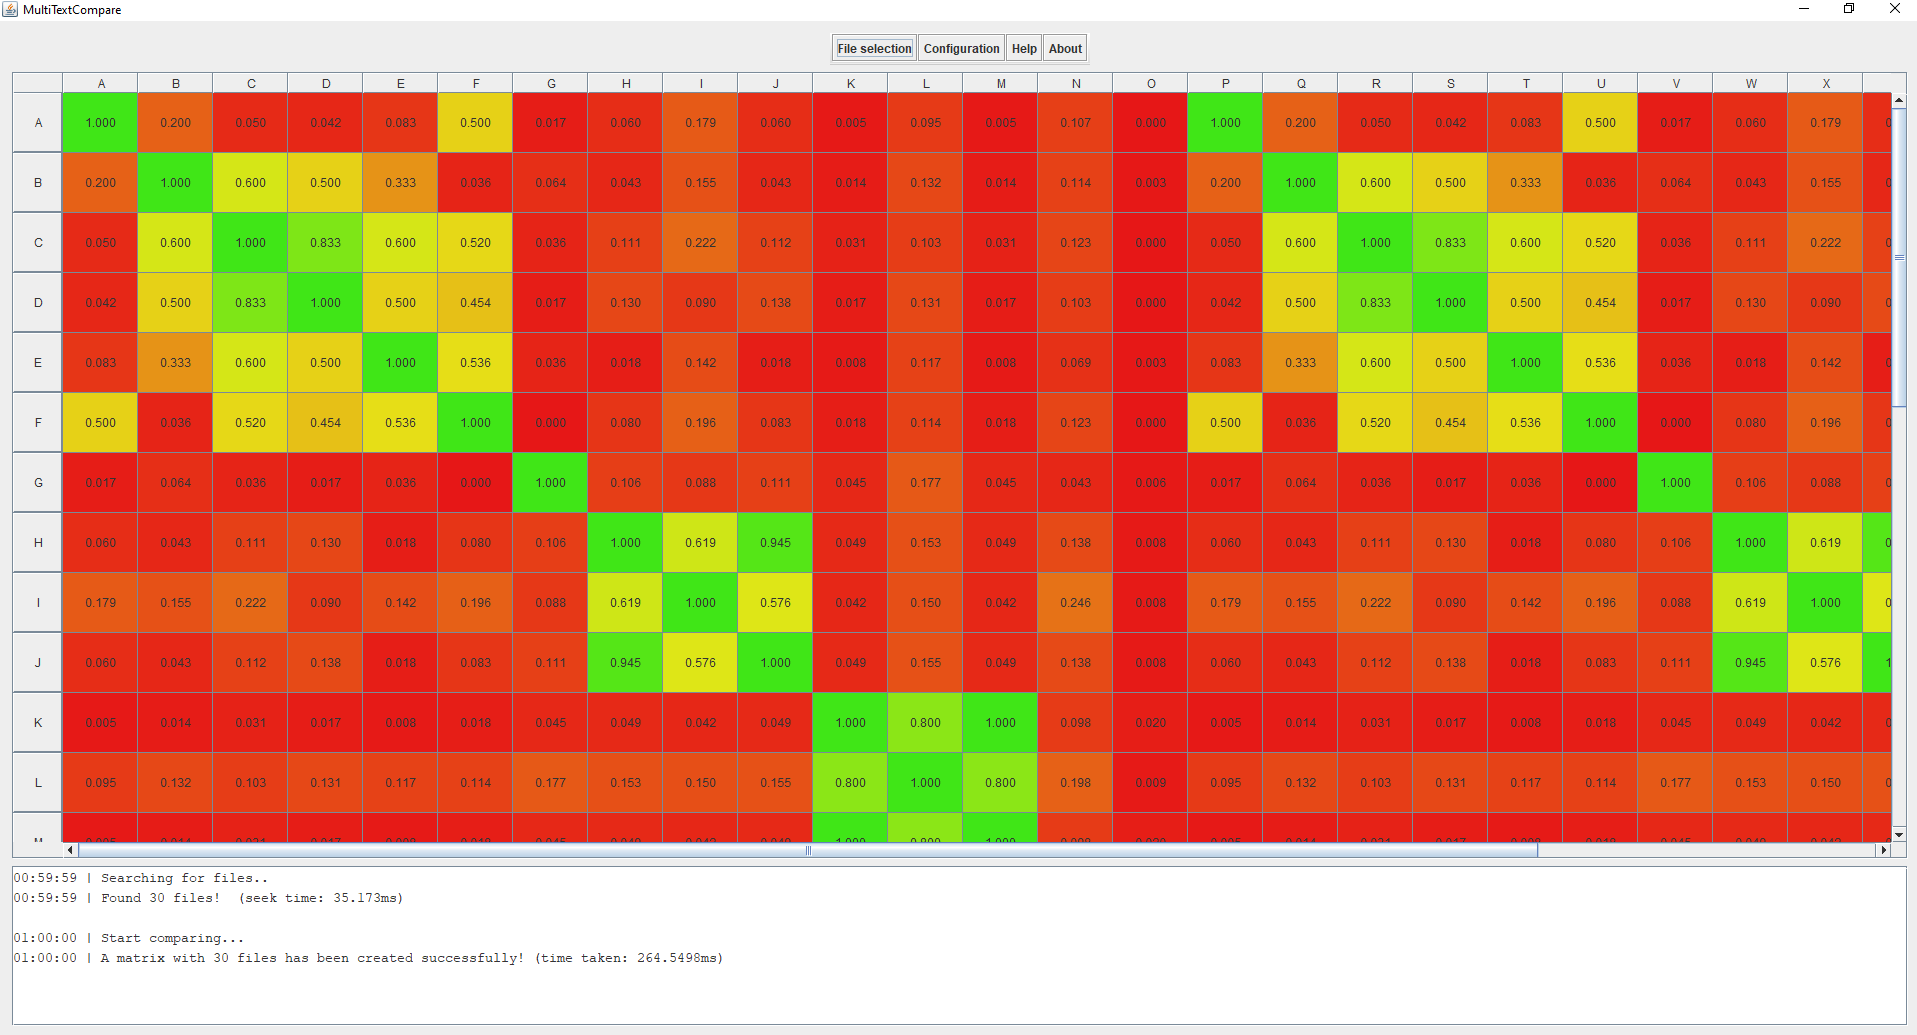
\includegraphics[scale=0.25]{images/matrix V1.png}
    \caption{Ähnlichkeitsmatrix in Version 1.0}
    \label{fig:matrix_v1}
\end{figure}

Zuletzt kann der Benutzer dann auf die einzelnen Zellen der Matrix klicken, um sich die Unterschiede für zwei oder drei Dateien gleichzeitig farbig markieren zu lassen. Dieser Stand der Software wird fortan als Version 1.0 referenziert.

\subsection{Zielsetzung}\label{zielsetzung}
Ziel dieser Arbeit ist es, die Software MultiTextCompare an den nötigen Stellen zu verbessern. Dazu zählen hauptsächlich die Benutzerfreundlichkeit, Laufzeit und die Genauigkeit der Vergleichsalgorithmen.

Dabei gliedert sich die Arbeit in 6 Kapitel: Die theoretischen Grundlagen, die Konzeption der Software, die Implementierung der Verbesserungen, deren Verifikation sowie die Zusammenfassung mit Ausblick.

Die theoretischen Grundlagen sollen zunächst in das Thema des Textvergleichs einleiten. Dafür wird der Begriff der Ähnlichkeit von Zeichenketten diskutiert und anhand von zwei verschiedenen Textvergleichsalgorithmen dargestellt. Darauf folgt eine Übersicht zu den Dateiformaten \acrshort{xml} und \acrshort{json} und eine Vorstellung der speziellen Aspekte in der Programmierung der Software. Dort geht es dann beispielsweise um die Funktionsweise des UI-Toolkits Java Swing und die Implementierung von Nebenläufigkeit in Java.

Das Kapitel zur Konzeption zieht anschließend einen Vergleich zu bereits bestehender Software, deren Vorteilen und ihren Limitationen. Danach werden kurz die besonderen Aspekte für die Entwicklung dargestellt. Darunter liegen bspw. die zu verwendenden Bibliotheken und Tools und die Limitationen der Systeme auf denen die Software lauffähig sein soll. Zuletzt gibt es einen kurzen Überblick über die bestehende Architektur der Software und der Codebase.

In Kapitel 4 geht es hauptsächlich um die durchzuführenden Aufgaben dieser Arbeit. Es wird also konkret die Vorgehensweise bei der Entwicklung erklärt. Dabei soll auch gezeigt werden, durch welche Probleme eine Änderung der Funktionalität notwendig ist, und wie diese Probleme gelöst werden können. Für die Dateiformate \acrshort{xml} und \acrshort{json} sollen zudem eigene Vergleichsalgorithmen entworfen werden, die nun nicht mehr auf reiner Textbasis arbeiten, sondern sich explizit mit den Baumstrukturen der Dokumente auseinandersetzen, um dort einen spezialisierten Vergleich durchführen zu können.

Das fünfte Kapitel beschäftigt sich dann ausführlich mit der Verifikation der in Kapitel 4 durchgeführten Laufzeitoptimierungen und den neuen Vergleichsalgorithmen. Dabei werden die Testsysteme vorgestellt, die Methodik erklärt und die Ergebnisse kritisch evaluiert.

Im letzten Kapitel befindet sich abschließend eine Zusammenfassung der durchgeführten Entwicklungen und der gewonnenen Erkentnisse und ein Ausblick, wie die Software in Zukunft noch weiter verbessert werden könnte.